% !TEX root = ../../Lazcorreta.Tesis.tex

Observar el comportamiento de los individuos de cierta población, anotarlo y analizarlo buscando \patrones de comportamiento que permitan conocer mejor a dicha población es uno de los métodos más utilizados por la ciencia desde sus inicios. El objetivo de esta metodología es siempre el mismo: transformar \textsl{datos} en \textsl{conocimiento}, \textsl{experiencia} en \textsl{ciencia}. Las Matemáticas y la Estadística han aportado sus cimientos, contando con las necesidades y experiencias de las demás ciencias para modelizar correctamente los datos observados de modo que puedan ser analizados científicamente. La Informática aportó el \kdd (\KDD) como paradigma de Descubrimiento de Conocimiento en \dbs (\DB), que derivaron en la \dm (\DM) ante el crecimiento exponencial de contenido en las \DB. Con la ayuda de la Telemática, junto a todas las ciencias que han impulsado su brutal crecimiento desde hace unas décadas, las ciencias de la tecnología proporcionan herramientas eficientes para la captación masiva de datos, su almacenamiento y su distribución. Uno de los objetivos de la ciencia actual, apoyada por la tecnología, es extraer en tiempo real el conocimiento que contienen esas grandes cantidades de datos.

\citet{FayyadPiatetskySmyth-FromDataMiningToKnowledgeDiscoveryInDatabases-1996} definieron el proceso de \kdd como "`\emph{El proceso no trivial de identificar \patrones de datos válidos, novedosos, potencialmente útiles y comprensibles}"'. La figura~\ref{fig:fasesProcesoKDDFayyad}, extraída de su artículo, muestra una idea del proceso completo de \KDD, formado por cinco fases recurrentes que permiten convertir los \textsl{datos disponibles} en \textsl{conocimiento}. Una \textsl{selección} de los datos disponibles convenientemente \textsl{preprocesados} y \textsl{transformados} pueden ser sometidos a técnicas de \dm que descubran los \patrones que contienen para ser convertidos en conocimiento. \citet{Friedman-DataMiningAndStatisticsWhatIsTheConnection-1997} considera el proceso de \KDD como un análisis exploratorio de datos para grandes \dbs. Hay muchos autores que describen a su modo las diferentes fases del proceso de \KDD~\citep{RokachMaimon-DataMiningWithDecisionTreesTheoryAndApplications2nd-2014}, siguiendo todos ellos la propuesta de Fayyad.
\begin{figure}[htbp]
	\centering
		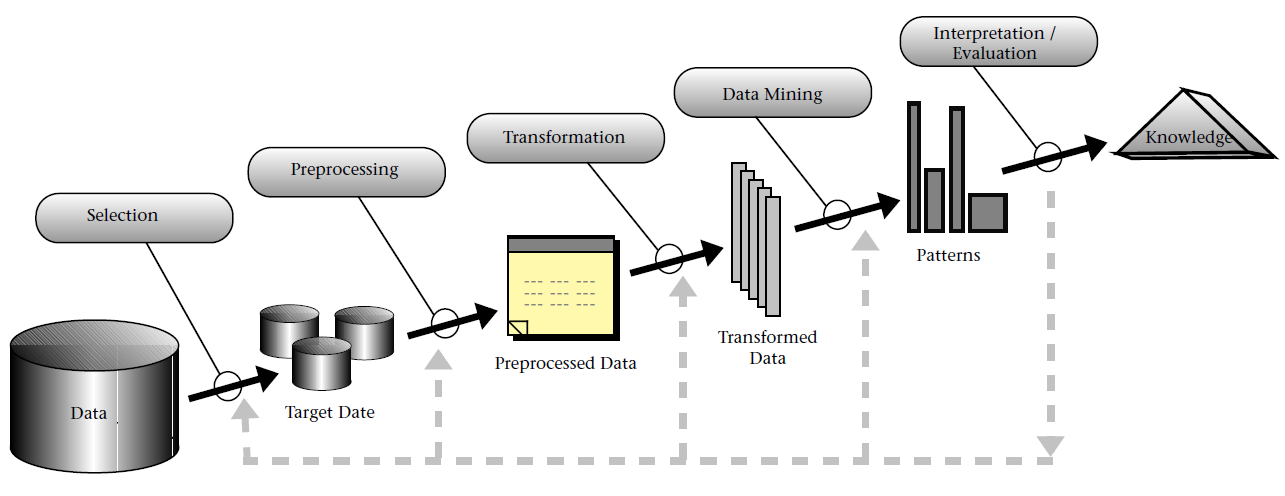
\includegraphics[width=\textwidth]{fasesProcesoKDDFayyad}
	\caption{Fases del proceso de \KDD [Fayyad et al. (1996)]}
	\label{fig:fasesProcesoKDDFayyad}
\end{figure}

Un \sr (\SR) es un claro ejemplo del proceso de \KDD. Se basa en la capacidad de almacenamiento y procesamiento que ofrece la tecnología, con estrategias diseñadas por expertos en su área (selección, preprocesamiento, transformación y análisis), y el objetivo de hacer recomendaciones de calidad de forma semi-automática en base a los \patrones obtenidos.

Tradicionalmente ha sido una persona quien realizaba todo el proceso de captación de datos, análisis y conversión en conocimiento. Un típico ejemplo es el del médico que ha estudiado una carrera para conocer la experiencia de otros científicos en el mismo campo, al ejercer ha recabado datos sobre la salud de sus usuarios, los pacientes, realiza un análisis exponiendo los datos obtenidos a la experiencia (propia o derivada de sus estudios o comunicaciones con otros expertos) y cuando encuentra un \patron de comportamiento que se adapte al paciente al que está tratando emite un diagnóstico junto a una recomendación.

De un \sr se espera precisamente esto, que convierta la información en conocimiento en base a comparar los datos de un individuo con \patrones de comportamiento ya contrastados en la población a la que pertenece el individuo. Cuando esta población es muy dinámica (las enfermedades a que se enfrentan los médicos no son siempre conocidas o pueden evolucionar de modo que ya no sea válido el conocimiento previamente adquirido) el proceso se ha de repetir cíclicamente aportando nuevos datos o conocimiento o renunciando a aquellos que no aporten valor al conocimiento final. Son muchas las disciplinas que se han sumado a la búsqueda de \srs que se auto-gestionen, como la aportación de~\citet{KourisMakrisTsakalidis-UsingIR-2005} utilizando métodos y técnicas de \emph{Recuperación de la Información}.

Con la tecnología actual se espera que esta conversión sea de gran calidad y en tiempo real ya que se conocen muchos datos y se pueden analizar desde múltiples perspectivas mediante procesos informáticos muy rápidos. Esta expectativa se manifiesta en la gran cantidad de trabajos científicos que hacen su aporte para la obtención de \srs en casi todas las áreas de investigación. Volviendo a nuestro médico, podríamos decir que es un \SR y cuanta más experiencia tenga (propia o ajena, pero de calidad) más rápidos y certeros serán sus diagnósticos y, por tanto, sus recomendaciones. Si nuestro médico utiliza la tecnología actual llegará un momento en uno de sus análisis en que querrá conocer nuevos datos de su paciente, otro investigador puede averiguar con qué dispositivo se pueden obtener los nuevos datos, otro investigador estudiará la influencia de este nuevo dato sobre el diagnóstico y si los resultados son "`correctos"' se puede implementar un sistema que realice de forma automática este proceso en tiempo real, con el coste de utilizar mayor cantidad de datos.

Ya hace más de dos décadas~\citet{FrawleyPiatetskyMatheus-KDDOverview-1992} estimaban que la cantidad de información almacenada de forma digital se duplica cada 20 meses. Con los avances tecnológicos sobre digitalización, almacenamiento y transmisión de datos y su enorme abaratamiento estas estimaciones se quedan cortas hoy en día por lo que hay que seguir investigando el modo de analizar de forma eficiente cada vez más grandes cantidades de datos.%\footnote{En esa época la digitalización de datos era básicamente manual, hoy en día todos tenemos dispositivos capaces de adquirir datos de diferentes fuentes y guardarlos o transmitirlos a otros dispositivos de múltiples modos.}

Los \srws (\SRW) son un caso particular de los \srs, están más adaptados a la fase de recolección de datos que cualquier otro \SR porque se usan únicamente con dispositivos informáticos unidos telemáticamente. Cada vez que un usuario utiliza un servicio web está enviando datos a un servidor, datos que el servidor puede almacenar en sus discos duros o en su memoria RAM para ser analizados inmediatamente o con posterioridad (generalmente se harán ambos análisis). Si el \SRW ya "`conoce"' lo que suele hacer un determinado usuario de su sitio web puede mejorar su \ux (\UX) facilitándole enlaces de forma dinámica para que el usuario cumpla su objetivo con el menor esfuerzo posible. Si el sistema no conoce al usuario puede comparar su comportamiento con el del resto de usuarios del sitio web, si encuentra un \patron de comportamiento que se adapte al usuario desconocido también podrá mejorar su \UX. Sin embargo el crecimiento de información en la web es cada día mayor, llegando a cotas que hacen muy complejo el planteamiento expuesto.

\citet{Etzioni-TheWWWQuagmireOrGoldMine-1996} planteó ideas sobre la pobre utilización de la gran cantidad de datos que contienen y recogen los servidores web. Estaba emergiendo la \wm bajo tres perspectivas: \wsm, \wcm y \wum. Conociendo el contenido de la web, cómo está estructurado y cómo se usa se podría llegar a niveles altísimos de personalización de la web. Aplicando el conocimiento adquirido a través de estas tres perspectivas al uso de la web se podrían desarrollar \srws que operasen en tiempo real sobre todos los usuarios de la web, recogiendo nuevos datos de uso y analizándolos para obtener mejores resultados, conocimiento de mayor calidad y mejores recomendaciones.

\citet{ChoKimKim-PersonalizedRecommenderSystem-2002} proponen su propio \srw para un e-comercio basándose en \wum, inducción de árboles de decisión, \arm y una taxonomía del producto comercializado. Cada vez tenemos más técnicas a disposición de la \KDD y esto generará un flujo constante de investigaciones sobre esta materia. Al analizar los datos de uso de la \WWW se pueden hacer análisis más precisos sobre los intereses o preferencias de los usuarios.

\citet{SchaferKonstanRiedl-ECommerceRecomendation-2001} presentan una taxonomía sobre \srs centrándose en portales de e-comercio. Las técnicas a usar para personalizar las recomendaciones puede depender de muchos factores, entre los que podríamos citar:
\begin{itemize}
  \item Las recomendaciones pueden estar dirigidas a usuarios específicos o a todos los usuarios del servicio.
  \item El objetivo de la recomendación puede ser predecir cuánto le gustará el producto recomendado a cierto usuario o bien obtener una lista de productos de alto interés para el usuario (problema de las top-$N$ recomendaciones)
  \item Se puede tener preparada la recomendación u obtenerla bajo demanda, en cuyo caso la eficiencia de los algoritmos utilizados adquiere gran importancia.
\end{itemize}

Al iniciar nuestra investigación queríamos implementar un \srw basado en el conocimiento adquirido mediante la aplicación de técnicas de \wum a los datos recogidos en un \flog por un servidor web. Había ya mucha investigación al respecto y comenzamos a seleccionar artículos de investigación sobre la \WUM como una realización específica de un proceso de \KDD.

En las siguientes secciones describiremos las fases mostradas en la figura~\ref{fig:fasesProcesoKDDFayyad} con el enfoque utilizado en este trabajo, la \wum, haciendo una visión global de los \SRW y profundizando en los aspectos que más afectan al proceso de investigación mostrado en este informe.
